\section{Neural Network (NN)}\label{s:neural_network}
Another popular way of solving the problem is through the use of Artificial Intelligence~(AI)~\cite{Ciresan2010}. AI is, at the time of writing, a hot topic with Artificial Neural Networks (ANN) receiving special attention.
In this section, a simple feedforward neural net will be created to attempt the classification of the digit from the data set.
The neural net created by Higham will be taken as a basis~\cite{Higham2018}.
The XOR problem based on the logical exclusive-or operator is a test problem that will be solved to showcase the different elements of a neural network~\cite{Shiffman2018}.

In Section~\ref{s:nn:structure} the structure of a neural network is explained.
Section~\ref{s:fp} contains information about forward propagation, followed by the loss function in Section~\ref{s:loss}.
The way a neural network is trained can be found in Section~\ref{s:training}.
The choices for the example problem are motivated in Section~\ref{s:xor}. Section~\ref{s:perf} analyses the results of the neural network that solves the XOR problem.
Finally, the discussed concepts are applied to the classification problem in Section~\ref{s:digit_recognition}.

\subsection{Structure}\label{s:nn:structure}
There are many different complex structures such as recurrent or convolutional neural networks, however for simplicity we will focus on a feedforward neural network.
A feedforward neural network has two main components: nodes, often called neurons, and edges.
A node can have a value which is dependent on the values of nodes connected to it, the weights of the edges, and optionally the bias.
Typically, these artificial neurons are aggregated into layers (see Figure~\ref{fig:neural_net}).

The first layer is called the input layer.
This layer contains the input neurons, which are the neurons with a direct correspondence to the input.
The last layer is called the output layer.
The calculated values in the output neurons are the final result and thus output of the neural network.
All other layers are called hidden layers as their functionality is not exposed to the user.
In the example, illustrated by Figure~\ref{fig:neural_net}, there is only one hidden layer.
\def\layersep{5.3cm}
\begin{figure}[H]
    \centering
    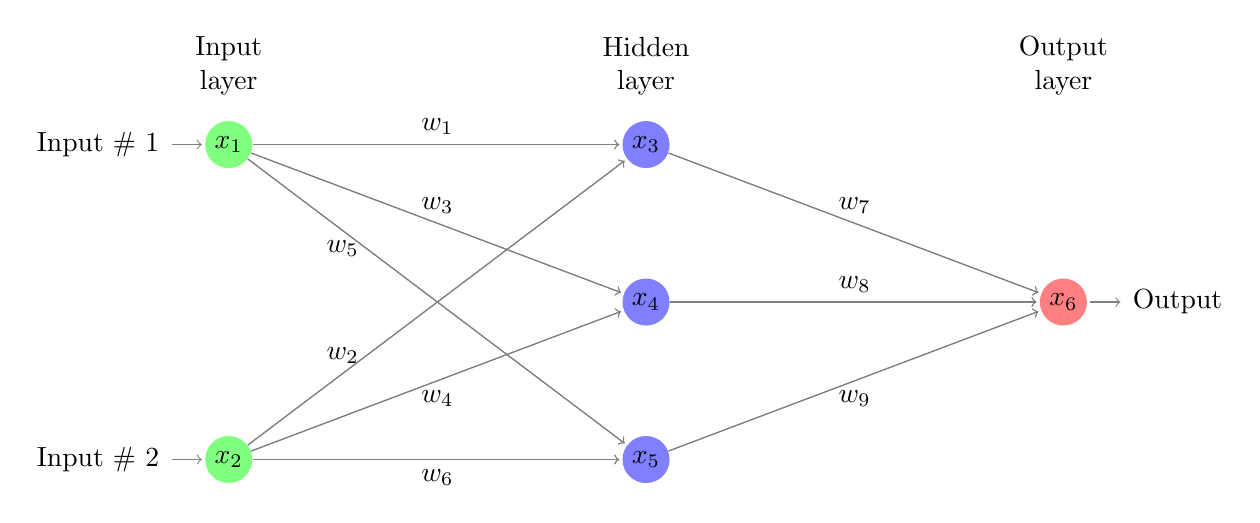
\begin{tikzpicture}[shorten >=1pt,->,draw=black!50, node distance=\layersep]
      \tikzstyle{every pin edge}=[<-,shorten <=1pt]
      \tikzstyle{neuron}=[circle,fill=black!25,minimum size=17pt,inner sep=0pt]
      \tikzstyle{input neuron}=[neuron, fill=green!50];
      \tikzstyle{output neuron}=[neuron, fill=red!50];
      \tikzstyle{hidden neuron}=[neuron, fill=blue!50];
      \tikzstyle{annot} = [text width=4em, text centered]
  
      % Draw the input layer nodes
      \foreach \name / \y in {1,...,2}
      % This is the same as writing \foreach \name / \y in {1/1,2/2,3/3,4/4}
          \node[input neuron, pin=left:Input \# \y] (I-\name) at (0,4*-\y + 3) {\(x_{\y}\)};
  
      % Draw the hidden layer nodes
      \foreach \name / \y in {3,...,5}
          \path[yshift=1cm]
              node[hidden neuron] (H-\name) at (\layersep,2*-\y + 4) {\(x_{\y}\)};
  
      % Draw the output layer node
      \node[output neuron,pin={[pin edge={->}]right:Output}, right of=H-4] (0) {\(x_6\)};
  
      % Connect every node in the input layer with every node in the
      % hidden layer.
      \foreach \source in {1,...,2}
          \foreach \dest in {3,...,5}
              \path (I-\source) edge (H-\dest);
  
      % Connect every node in the hidden layer with the output layer
      \foreach \source in {3,...,5}
          \path (H-\source) edge (0);
  
      % Annotate the layers
      \node[annot,above of=H-3, node distance=1cm] (hl) {Hidden layer};
      \node[annot,left of=hl] {Input layer};
      \node[annot,right of=hl] {Output layer};
      \draw (I-1) -- (H-3) node[midway, above]{\(w_1\)};
      \draw (I-2) -- (H-3) node[near start, above]{\(w_2\)};
      \draw (I-1) -- (H-4) node[midway, above]{\(w_3\)};
      \draw (I-2) -- (H-4) node[midway, below]{\(w_4\)};
      \draw (I-1) -- (H-5) node[near start, below]{\(w_5\)};
      \draw (I-2) -- (H-5) node[midway, below]{\(w_6\)};
      \draw (H-3) -- (0) node[midway, above]{\(w_7\)};
      \draw (H-4) -- (0) node[midway, above]{\(w_8\)};
      \draw (H-5) -- (0) node[midway, below]{\(w_9\)};
  \end{tikzpicture}


    \caption{Neural network.}\label{fig:neural_net}
\end{figure}
The sizes of the input and output layers are often largely dictated by the problem that you are trying to solve.
Generally, deciding on the number of hidden layers and the number of nodes within each layer is not an exact science.
Rules of thumb have been suggested, however there is no widely accepted technique~\cite{Higham2018}.

One property of a feedforward neural network is that edges can only be connected between two consecutive layers.
Consequently, the value of all nodes in the first layer need to be calculated, then the values in the nodes of the second layer and so on.
The process of calculating the nodes is aptly named forward propagation.

\subsection{Forward propagation}\label{s:fp}
First, forward propagation is illustrated on the XOR example.
Then, a more general formula is derived and some notation is introduced.

The input of a neural network consists of values.
The forward propagation of the example, seen in Figure~\ref{fig:neural_net}, goes as follows:
\begin{align*}
    x_1 & = \text{given by input}, & x_3 & = f(w_1\cdot x_1 + w_2\cdot x_2 + b_3), & x_6 & = f(w_7\cdot x_3 + w_8\cdot x_4+ w_9\cdot x_5 + b_6), \\
    x_2 & = \text{given by input}, & x_4 & = f(w_3\cdot x_1 + w_4\cdot x_2 + b_4),                                                               \\
        &                          & x_5 & = f(w_5\cdot x_1 + w_6\cdot x_2 + b_5),
\end{align*}

Notice that these equations can easily be written in matrix form.
These matrices will be referred to as the weight matrices.
This yields the following:
\begin{align*}
    \begin{pmatrix}
        x_3 \\x_4\\x_5
    \end{pmatrix}
    =
    f\left(
    \begin{pmatrix}
        w_1 & w_2 \\
        w_3 & w_4 \\
        w_5 & w_6
    \end{pmatrix}
    \begin{pmatrix}
        x_1 \\x_2
    \end{pmatrix}
    +
    \begin{pmatrix}
        b_3 \\b_4\\b_5
    \end{pmatrix}
    \right), &  &
        x_6
    =
    f\left(
    \begin{pmatrix}
        w_7 & w_8 & w_9
    \end{pmatrix}
    \begin{pmatrix}
        x_3 \\ x_4\\ x_5
    \end{pmatrix}
    +
        b_6
    \right).
\end{align*}

A simple substitution yields the following expression for computing the output in a single step:
\[
        x_6
    =
    f\left(
    \begin{pmatrix}
            w_7 & w_8 & w_9
        \end{pmatrix}
    f\left(
        \begin{pmatrix}
                w_1 & w_2 \\
                w_3 & w_4 \\
                w_5 & w_6
            \end{pmatrix}
        \begin{pmatrix}
                x_1 \\x_2
            \end{pmatrix}
        +
        \begin{pmatrix}
                b_3 \\b_4\\b_5
            \end{pmatrix}
        \right)
    +
            b_6
    \right).
\]

The function \(f\) is called the activation function.
Popular choices for this function are the linear function \(f(x) = x\), the Rectified linear unit (ReLU) function \(f(x) = x\cdot\mathbbm{1}\{x > 0\} \), and the sigmoid function \(f(x) = \sigma(x) = 1/(1+e^{-x})\)~\cite{Higham2018}.
Furthermore, the XOR problem has outputs that can be divided into two classes, true and false, making it a classification problem.
We will take the sigmoid function as the activation function as it is typically chosen in case of classification problems.

For use further in this paper, a general formula is useful.
A general formula is thus derived and some notation is introduced.
Let \(\ell \) be a number corresponding to a layer, let \(\vec{W}^{[\ell]}\) be the weight matrix of layer from layer \(\ell - 1\) to \(\ell \), and let \(\vec{b}^{[\ell]}\) be the biases of layer~\(\ell \).
We define the weighted input of layer \(2 \leq \ell \leq L \) before and after the activation function to be
\begin{align*}
    \vec{z}^{[\ell]} & = \vec{W}^{[\ell]}\vec{a}^{[\ell - 1]} + \vec{b}^{[\ell]}, \\
    \vec{a}^{[\ell]} & = f\left(\vec{z}^{[\ell]}\right),
\end{align*}
where \(L\) is the number of layers of the neural net and where \(a^{[1]}\) corresponds to the input.

The last, and arguably the most important, thing that is needed is a way to improve the weights and biases such that the network as a whole behaves as desired.
Changing the weights and biases for the purpose of improving performance is called training a neural network.
Before a network can be trained, a loss function needs to be computed.

\subsection{Loss function}\label{s:loss}
The loss function, also known as the cost function, is necessary to gauge the performance of the neural network.
A loss function takes the predicted output, \(x_p\in \{0, 1, \ldots, 9\} \), and the actual output, \(x_6\) as inputs and gives a measure of difference between the two.
In this paper the Mean Squared Error (MSE) is used, where \(n\) is the number of training samples.
The MSE is differentiable and has some other convenient properties, which made it very popular for feedforward neural networks such as this one.
The formula is displayed below.
\[C = \frac{1}{n}\sum_{i = 1}^n {(x_6 - x_p)}^2.\]

\subsection{Training the network}\label{s:training}
Training the network is the act of improving the weights and biases in such a way that the neural network behaves as desired.
The two ways discussed in this paper of improving these are through neuroevolution and back propagation.
Before the weights can be improved, initial weights need to be chosen.
There are several ways to pick these, however in this paper for the sake of simplicity they are initialised to a random number.
This can be any random number, however since very big or small values make the process slower we take random numbers from a normal distribution.

\subsubsection{Neuroevolution}
Neuroevolution (NE) is the artificial evolution of neural networks using Genetic Algorithms (GA).
GA are inspired by the process of natural selection.
Neuroevolution starts with creating several neural networks initialised with random weights and biases.
Then the models are tested on the training set and given a fitness score based on how well they performed.
The fittest neural networks have a chance to create so-called offspring, which is a new neural network with a combination of the parents weights and biases.
For each of the fittest there is also a chance to mutate, which randomly changes the weights by some small amount~\cite{Whitley1993}.

There are also more advanced NE algorithms such as the Neuroevolution with Augmenting Topology (NEAT).
Mutations with NEAT also include the possibility to change the topology or structure of the network~\cite{Stanley2002}.

\subsubsection{Gradient descent}
A popular way of improving an NN is through gradient descent with back propagation.
In Section~\ref{s:loss}, the loss function has been defined, which consists only out of the weights and inputs \(x_1, x_2\), and \(x_3\).
That makes this an optimisation problem, where the loss function needs to be minimised.
The calculation of the gradient requires the loss function to be differentiable and hence also continuous.
Even though there are solutions to solve this, however in this case this would add unnecessary complexity.
Differentiable activation functions are thus easier to work with and hence are generally preferred.

To make use of back propagation, first define the error in the \(j\)th neuron to be
\begin{align*}
    \delta^{[\ell]}_j = \frac{\partial C}{\partial z^{[\ell]}_j}, &  & \text{for } 2\leq j\leq n \text{ and }1 \leq j \leq n_\ell
\end{align*}
where \(n_\ell \) is the number of neurons in layer \(\ell \).
We point out that the usage of the term error is somewhat ambiguous.
The idea of referring to \(\delta^{[\ell]}_j\) as an error seems to have arisen because the cost function can only be minimum if all partial derivatives are zero, so \(\delta^{[\ell]}_j = 0\) is a useful goal.

Substituting the various formulas together with the chain rule, which can be found in the paper of Higham et al~\cite{Higham2018}, yields the following:\\
\textbf{Lemma~\cite{Higham2018}. }\textit{We have
    \begin{align}
        \vec{\delta}^{[L]}
         & = \sigma'(\vec{z}^{[L]})\circ (\vec{a}^L - \vec{x}_1),                                 \\
        \vec{\delta}^{[\ell]}
         & = \sigma'(\vec{z}^{[\ell]})\circ {(\vec{W}^{[\ell + 1]})}^T \vec{\delta}^{[\ell + 1]},
         & \textnormal{for }2\leq \ell \leq L -1,                                                 \\
        \frac{\partial C}{\partial w^{[\ell]}_{jk}}
         & = \delta^{[\ell]}_j a^{[\ell - 1]}_k,
         & \textnormal{for }2\leq \ell \leq L,\label{l:cw}                                        \\
        \frac{\partial C}{\partial b^{[\ell]}_j}
         & = \delta^{[\ell]}_j,
         & \textnormal{for }2\leq \ell \leq L.\label{l:cb}
    \end{align}}

Here, \(\circ \) also denotes the Hadamard or entrywise product.
Recall that in Section~\ref{s:fp} the input is propagated forward. This results in an output \(\vec{a}^L\), which corresponds to \(x_6\) in the XOR example.
The error of the output \(\bm{\delta}^{[L]}\) is computed.
Now, in a process called back propagation, the errors \(\bm{\delta}^{[p]}\) of the layer \(p\) with \(p = L - 1, \ldots, 2\) are calculated.
The error for layer \(1\) is not calculated as the input is given and cannot be changed with adjusting weights.

At this point a vector \(\bm{\delta}^{[\ell]}\) exists for each layer.
The last step to perform is to update the weights and biases using this vector and a single gradient descent step.
\begin{align*}
    \vec{W}^{[\ell]}_{new} &= \vec{W}^{[\ell]} - \eta \frac{\partial C}{\partial \vec{W}}^{[\ell]}\\ 
    &= \vec{W}^{[\ell]} - \eta \bm{\delta}^{[\ell]}\vec{a}^{[\ell - 1]}, && \text{see (\ref{l:cw}),}\\
    \vec{b}^{[\ell]}_{new} &= \vec{b}^{[\ell]} - \eta \frac{\partial C}{\partial \vec{W}}^{[\ell]}\\ 
    &= \vec{b}^{[\ell]} - \eta \bm{\delta}^{[\ell]}, && \text{see (\ref{l:cb}).}
\end{align*}

The symbol \(\eta \) is the learning rate or step size.
This learning rate influences how quickly the weights of the neural network are changed.
Generally, a lower learning rate results in slower training, however a larger learning rate will result in a change of weight values that is too large which means that the local minimum may never be obtained.
This is how gradient descent with the use of back propagation is applied to a neural network.

\subsection{XOR problem}\label{s:xor}
XOR stands for exclusive or, which is a logical operation that evaluates to true only when one of the inputs differ from each other~\cite{Simpson1987}.
The XOR is a logical operation, however the neural network is numerical, so an encoding must be chosen.
In this paper, true will be encoded with the number 1 and false with the number 0.
This yields the following inputs and corresponding outputs:
\begin{align*}
    \text{xor}\left(
    \begin{pmatrix}
            0 \\0
        \end{pmatrix}
    \right)
    =
    0, &  &
    \text{xor}\left(
    \begin{pmatrix}
            1 \\0
        \end{pmatrix}
    \right)
    =
    1, &  &
    \text{xor}\left(
    \begin{pmatrix}
            0 \\1
        \end{pmatrix}
    \right)
    =
    1, &  &
    \text{xor}\left(
    \begin{pmatrix}
            1 \\1
        \end{pmatrix}
    \right)
    =
    0,
\end{align*}
This example is chosen since the solution space is not linearly separable.
This means that there does not exist a single line that can divide the different classification outputs.
As a result, the problem cannot be solved by methods such as the single layer perceptron, hence making for a simple but non-trivial example~\cite{Shiffman2018}. The training set will then be the inputs with their corresponding labels. Normally, a proper subset of the input space is trained on, however in this case there are already such few solutions that all of the different input combinations are trained on.

In Figure~\ref{fig:xor} the reader can find the inputs with their corresponding labels. A blue cross means true, whereas a red circle means false.
For example, the exclusive-or operation on false and false yields false, hence a circle on \((0,0)\)
\begin{figure}[H]
    \centering
    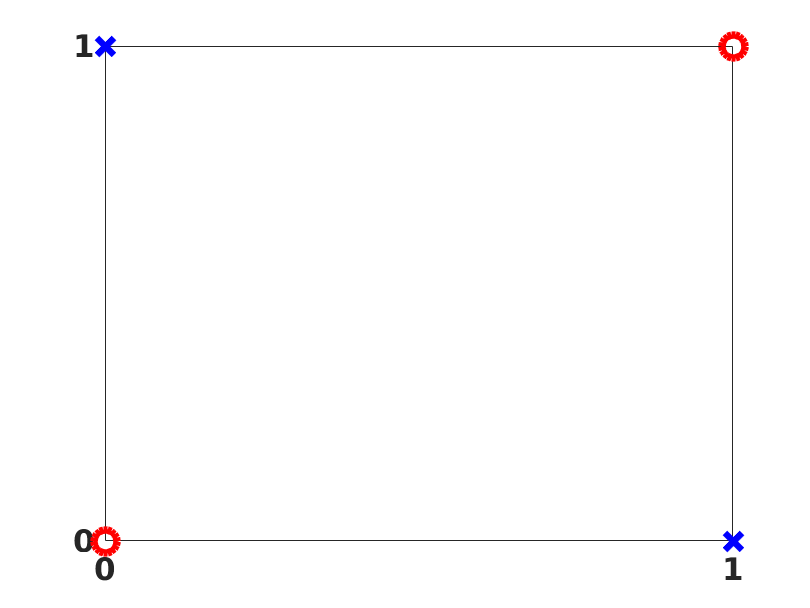
\includegraphics[width = .45\linewidth]{images/nn/xor.png}
    \caption{Output space of the encoded XOR operation.}\label{fig:xor}
\end{figure}
\subsection{Performance}\label{s:perf}
At this point all the necessary parts of a neural network are described.
The model is now trained, however we do not know when to stop training.
To do this the performance needs to be measured.
Based on those measurements it can be decided whether or not do another forward propagation followed by a back propagation step.

The training is done by simply cycling through the four possible inputs and training them.
This guarantees that all elements from the input space are equally important to the final neural network.
After adjusting the weights for a training input, the neural network is tested on a similar testing data set which it has not seen before.
The values of the loss function can then be plotted to see how the neural network is improving. In Figure~\ref{fig:xor_cost} this plot can be seen.

The test set used to calculate the loss in the plot is the same as the training set, so in this case the graph cannot be used to infer any useful information.
Figure~\ref{fig:xor_solved} visually represents the solution space, where a point in the grey areas is classified as a one, otherwise zero.
Since the points from the same class fall in the same coloured area, the conclusion can be made that the neural network behaves as desired.
\begin{figure}[H]
    \centering
    \begin{minipage}{0.45 \textwidth}
        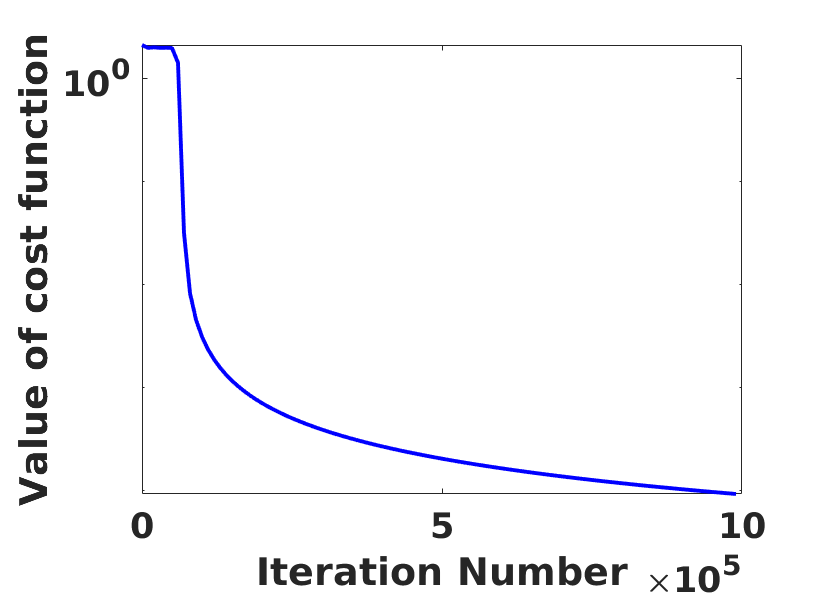
\includegraphics[width = \linewidth]{images/nn/xor_cost.png}
        \caption{Cost, or loss, function of the neural network over the number of iterations.}\label{fig:xor_cost}
    \end{minipage}
    \hspace{2em}
    \begin{minipage}{0.45 \textwidth}
        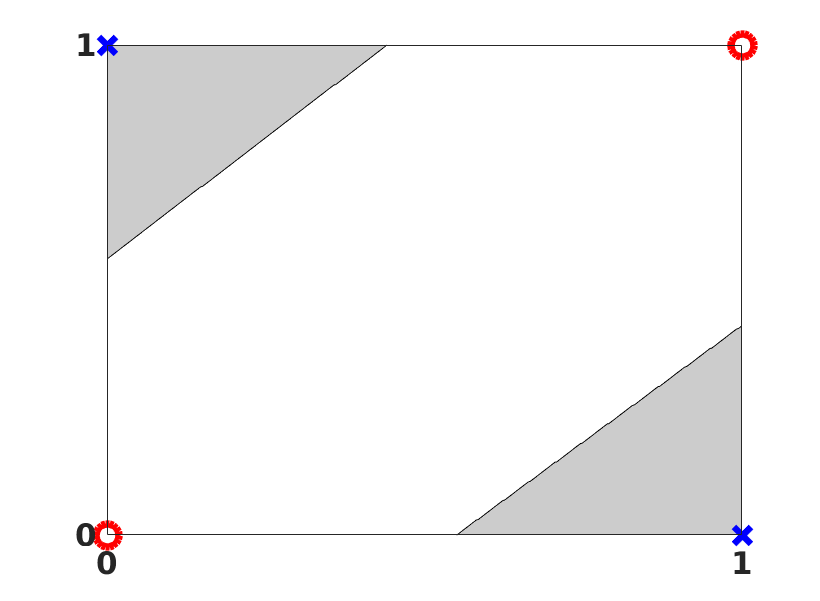
\includegraphics[width = \linewidth]{images/nn/xor_solved.png}
        \caption{Solution space of the neural net. All inputs in the grey areas will be classified as true, otherwise false.}\label{fig:xor_solved}
    \end{minipage}
\end{figure}

\subsubsection{Overfitting}
One notorious problem neural networks can have is overfitting. Overfitting produces a model that corresponds too closely to the training data set, and therefore fails to capture the desired behaviour~\cite{Hawkins2004}.
In case of the example, through Figure~\ref{fig:xor_solved}, the model is not overfitted.
This visualisation can only be made because the input dimensionality is two, so for higher dimensional inputs such as the image classification other methods need to be employed.

To deal with this when classifying digits, both the loss of the training set as well as the loss of the testing set is graphed. Overfitting then can be recognised if the loss of the training set continues to decrease while the loss of the test set does not~\cite{Higham2018}.

\subsection{Digit recognition}\label{s:digit_recognition}
The basic concepts of a neural network are explained through the use of the XOR example. To apply this to the problem of digit recognition, all important differences are highlighted and the necessary changes described.

\textbf{Structure:} The example has two nodes as inputs, while an image is a vector \(\vec{x}\in\mathbb{R}^{256}\), so the input layer now has 256 nodes.
The output is now one of 10 classes from 0 to 9.
Hence, the output is a vector \(\vec{y} \in \mathbb{R}^{10}\), where the first element corresponds to the confidence 0 is the correct answer, the second corresponds to 1 and so on~\cite{Higham2018}.
As for the hidden layers, a hidden layer with 64 then a hidden layer with 32 neurons is chosen.
This structure is an estimated guess as there are no clear rules for the structure.

\textbf{Performance:} As mentioned in Section~\ref{s:perf}, the performance in the form of time and accuracy will now be measured on a separate test set, while plotting the error of the training set to make sure the model is not overfitted.

At this point the model is trained with the MSE of the data plotted in Figure~\ref{fig:mse_data} and the accuracy plotted in Figure~\ref{fig:acc_data}.
As can be seen in Figure~\ref{fig:acc_data}, the MSE of the training data is nearly zero without overfitting.
This difference suggests that more training data would increase the performance of the neural network as the training data has an accuracy near one, while there is no overfitting present.

\begin{figure}[H]
    \centering
    \begin{minipage}{0.45\textwidth}
        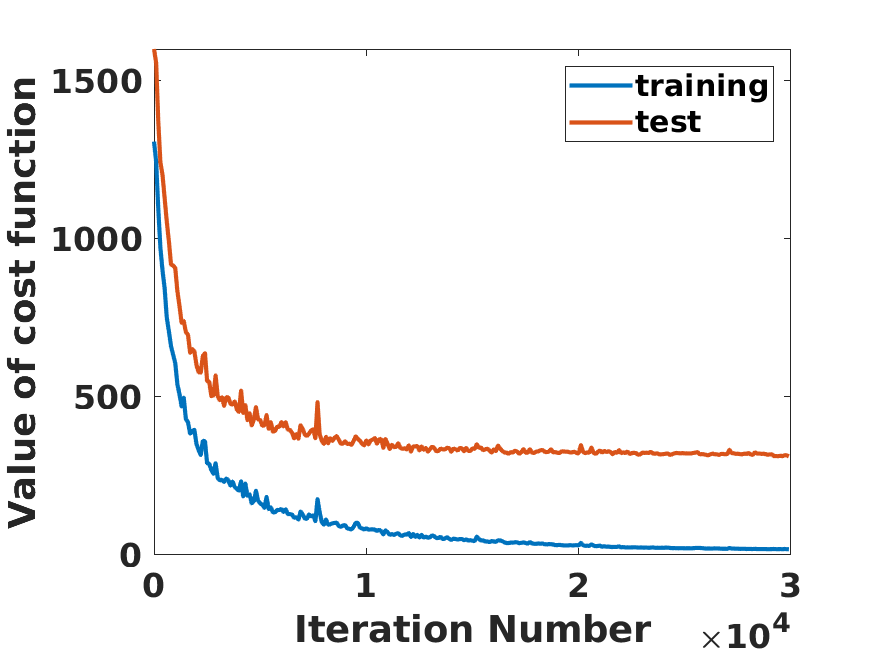
\includegraphics[width = \textwidth]{images/nn/mse_data.png}
        \caption{MSE of test and training data.}\label{fig:mse_data}
    \end{minipage}
    \hspace{2em}
    \begin{minipage}{0.45\textwidth}
        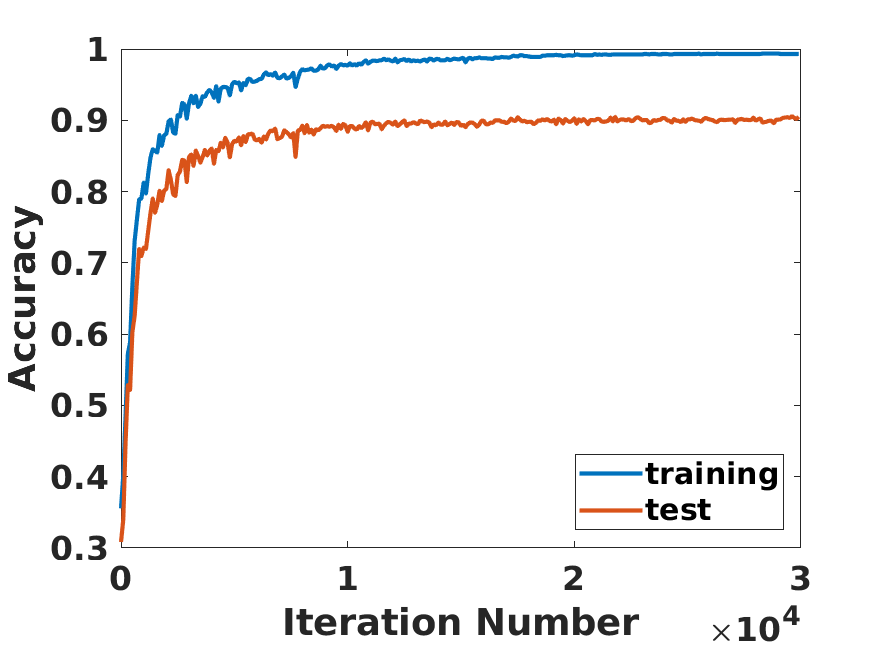
\includegraphics[width = \textwidth]{images/nn/acc_data.png}
        \caption{Accuracy of test and training data.}\label{fig:acc_data}
    \end{minipage}
\end{figure}

In Figure~\ref{fig:acc_data}, the number of iterations is directly proportional to the amount of time used. In Table~\ref{tab:neural_results}, a few points are sampled with the respective duration for that run. Concluding, the point where the variation is bigger than the improvement is around \(2\cdot10^4\) number of iterations.

\begin{table}[H]
    \centering
    \caption{Results of the neural network on the data set.}\label{tab:neural_results}
    \begin{tabular}{c c c c}
        \toprule
        \textbf{Accuracy}         & 0.893           & 0.905           & 0.900           \\
        \textbf{Number of iterations} & \(1\cdot 10^4\) & \(3\cdot 10^4\) & \(9\cdot 10^4\) \\
        \textbf{Time (s)}             & 0.52            & 1.10            & 4.31            \\
        \bottomrule
    \end{tabular}
\end{table}

It is important to note that the neural network, just like the SVD, has a fixed classification time.
As mentioned earlier, the model could be improved by adding a lot more training data as the current training data gets a classification accuracy of nearly one.
These facts combined make for a model that after the initial training period can get very accurate while having a short classification time.

We have now seen all the different techniques and in the next section some conclusions will be drawn.